%%%%%%%%%%%%%%%%%%%%%%%%%%%%%%%%%%%%%%%%%%%%%%%%%%%%%%%%%%%%%%%%%%%%%%%%%%
%% SECTION ONE
%%%%%%%%%%%%%%%%%%%%%%%%%%%%%%%%%%%%%%%%%%%%%%%%%%%%%%%%%%%%%%%%%%%%%%%%%%

\chapter{The Spectral Gap of Reversal Graphs}

\section{Introduction}


Consider a permutation $\tau$ in the symmetric group $S_n$, written in 
word notation $(\tau_1, \tau_2, \cdots, \tau_n)$, where we denote $\tau(i) = \tau_i$.  
A \textit{substring} is a subsequence of $\tau$, $(\tau_i, \tau_{i+1}, \ldots, \tau_j)$,
for some $1 \leq i < j\leq n$, and \textit{reversing} this substring yields
$(\tau_j, \tau_{j-1}, \ldots, \tau_i)$.
A \textit{substring reversal} of $\tau$ is any permutation obtained from $\tau$
by reversing a substring in $\tau$. 
Substring reversal is a well-studied operation on permutations, and 
often  appears in metrics on permutations, edit distances
and permutation statistics. There are numerous applications involving many variations of substring reversal,
such as genome arrangements and sequencing  (see \cite{BafnaPevzner1996}, \cite{Hannenhalli1996}, \cite{KececiogluSankoff1995}). 

The \textit{reversal graph} $R_n$ is the graph whose vertex set is the permutation group $S_n$, where
two vertices are adjacent if they are substring reversals of each other. Thus, $R_n$ has $n!$ vertices and is regular
with degree
$\binom {n} 2$.
Many properties of  the reversal graph $R_n$ have long been studied.
One interesting problem is to determine the minimum number of substring reversals needed to transform one
given permutation in $S_n$ to another, which is equivalent to finding 
a shortest path in $R_n$.  The smallest number of reversals required to turn any permutation into any other
is exactly the diameter of $R_n$, and 
it was shown in \cite{BafnaPevzner1996} that the diameter of 
the reversal graph is exactly $n-1$. The connectivity
and hamiltonicity of $R_n$ were investigated in \cite{LiMeng2008}. 
There are  still many questions concerning $R_n$ that remain unresolved. In this section, we examine
 the eigenvalues of  $R_n$, and determine the second largest eigenvalue of the adjacency matrix of $R_n$.
 Note that the second largest adjacency eigenvalue of a regular graph is intimately related to the
 rate of convergence for random walks on a graph. We use methods from graph coverings to determine
 the second largest eigenvalue of $R_n$, although our techniques cannot be used to determine
 the whole spectrum of $R_n$.



 An intriguing variation of substring reversal is  {\it prefix reversal} (or {\it pancake flipping}) where only
 substrings of the form $(\tau_1, \ldots, \tau_j)$ are allowed to be reversed.
The \textit{prefix reversal graph}, or  the \textit{pancake graph}, $\mathcal{P}_n$ 
is a special subgraph of $R_n$.  ${\mathcal P}_n$  also has vertex set $S_n$  but
the edge set is  restricted. In $\mathcal{P}_n$, the 
neighbors of $\tau$ are the permutations of the form  
 \[ (\tau_k, \tau_{k-1}, \cdots, \tau_1, \tau_{k+1}, \cdots, \tau_n) \]
for $1 < k \leq n$.
 In contrast to the reversal graph
where the exact value of the diameter is known, the problem of determining the diameter of the pancake  
graph has a long history and still remains open.
This problem was first posed by Jacob Goodman, under the pseudonym Harry Dweighter, as a Monthly problem
in 1975 \cite{Dweighter1975}.
The current best upper bound is $f(n) \leq \frac{18}{11} n $, due to
Chitturi et al. \cite{ChitturiEtAl2009}, improving on a previous bound of $\frac{5}{3} n$ given by
 Gates and Papadimitriou \cite{GatesPapadimitriou1979} in 1979.  The best lower bound is
$f(n) \geq 15 \left\lfloor \frac{n}{14} \right\rceil$, which is due to 
Heydari and Sudborough \cite{HeydariSudborough1997}.  Recently it was shown that the problem of  determining the exact minimum number of flips
to transform  one permutation $\tau_1$ into another permutation $\tau_2$, for two
given permutations $\tau_1$ and $\tau_2$, is NP--hard \cite{BulteauEtAl2015}.
  In \cite{Cesi2009}, it 
was determined that the spectral gap of $\mathcal{P}_n$ is one, answering a 
question posed in \cite{GunnellsEtAl2007}.
We will determine the spectral gaps for a family of graphs which contains certain Cayley graphs
including $\mathcal{P}_n$, giving an alternative proof in that case.
We then use the spectral gap of $\mathcal{P}_n$, together with a decomposition of $R_n$
into $P_n$ and copies of $R_{n-1}$, to determine the second largest
eigenvalue of $R_n$.


\begin{theorem}\label{thm:rev_eig}
 If $\mu_1, \mu_2$ are the two largest eigenvalues of the adjacency matrix
 of $R_n$, then  
 \[  \mu_1 = \binom{n}{2}, \text{ and } \mu_2 = \binom{n}{2}-n. \]
\end{theorem}



We will consider a family of graphs that generalizes the pancake graph, 
and show that for every graph in this family the spectral gap is one. 

\begin{theorem}\label{thm:main}
 Let $\mathcal{F}_n$ be the set of all graphs whose vertex set is the symmetric
 group $S_n$, and where for each vertex $\tau$ and each $2 \leq i \leq n$, 
 $\tau$ is adjacent to exactly one vertex of the form 
 \[ (\tau_i, \alpha_2, \alpha_3, \cdots, \alpha_{i-1}, \tau_1, \tau_{i+1}, \cdots, \tau_n). \]
 That is, the first and $i$th entries are swapped, and the entries in between are possibly rearranged.
 Then for any graph $G \in \mathcal{F}_n$, the two largest eigenvalues of
 the adjacency matrix of $G$ are $n-1$ and $n-2$.  In particular, the 
 adjacency spectral gap of $G$ is $1$.
\end{theorem}

The graphs $R_n$ and $\mathcal{P}_n$, as well as many of the graphs in 
$\mathcal{F}_n$, are Cayley graphs of the symmetric group $S_n$.
Indeed, Cayley graphs of the symmetric group  
have been the subject of extensive study,
with particular interest in their spectral gap.  In \cite{Lubotzky1995}, 
Lubotzky posed the problem of finding a family of $k$-regular Cayley
graphs of $S_n$ with spectral gap bounded away from zero;  an explicit
construction of such a family was found in \cite{Kassabov2007}.  For many 
particular Cayley graphs of $S_n$, the spectral gap has been computed
\cite{Friedman2000,FlattoEtAl1985,Cesi2009},
and the case when $S$ consists of transpositions is particularly well-studied.
Of particular relevance here, the Cayley graph with generating set
\[S = \{(1\ k) : 2 \leq k \leq n\}\] 
belongs to the family $\mathcal{F}_n$, and
the spectral gap was determined to be $1$ in \cite{FlattoEtAl1985}.


The remainder of the paper is organized as follows.  In Section 2 we review
the necessary background and establish notation.  In Section 3 we recall
the notions of graph coverings and projections, which we will use frequently 
in our proofs.  In Section 4 we introduce a graph which is a projection
of every graph in the family $\mathcal{F}_n$, which provides a lower bound of one
on the spectral gap of every graph in this family.  We establish the corresponding upper bound in Section 5.
In Section 6 we prove Theorem~\ref{thm:rev_eig} and further investigate
the spectrum of $R_n$.  We conclude with some problems and remarks.



%%%%%%%%%%%%%%%%%%%%%%%%%%%%%%%%%%%%%%%%%%%%%%%%%%%%%%%%%%%%%%%%%%%%%%%%%%
%% SECTION TWO
%%%%%%%%%%%%%%%%%%%%%%%%%%%%%%%%%%%%%%%%%%%%%%%%%%%%%%%%%%%%%%%%%%%%%%%%%%

%\section{Preliminaries}
Before proceeding to define the graph spectra of interest here, we note that
the definitions of eigenvalues and eigenvectors are much simpler and cleaner for regular graphs
than those of weighted irregular graphs. Although the graphs 
$R_n$ and the graphs in $\mathcal{F}_n$, are regular, we will consider various
associated graphs which are irregular and weighted in order to determine the spectral
gap that we need.
Furthermore, we remark that the spectral gap of the adjacency matrix of a weighted or unweighted graph often depends
on a few of the largest degrees and therefore the spectral gap of the adjacency matrix  can {\it  not}
be used to determine the rate of convergence for random walks on irregular graphs.  Instead it is more appropriate
to study the combinatorial Laplacian and normalized Laplacian.
In this section, we consider general weighted graphs and define the eigenvalues of the normalized Laplacian,
which will be important when we define graph covers.
For undefined terminology, the reader is referred to  \cite{Chung1997}.


%We will use the following standard result from matrix analysis, see for 
%example \cite{HornJohnson}.  
%\begin{theorem}[Rayleigh--Ritz]\label{rayleigh}
%If $M$ is a Hermitian matrix, then the $k$th largest eigenvalue satisfies
% \[ \mu_k(M) = \max_{\textbf{v} \perp V_{k-1}} \frac{\textbf{v}^t M \textbf{v}}{\textbf{v}^t \textbf{v}}\]
%where $V_{k-1}$ is the vector space generated by $k-1$ eigenvectors 
%corresponding to the largest $k-1$ eigenvalues, and $V_0 = \emptyset$.
%\end{theorem}


Let $G$ denote a weighted undirected graph with edge weight $w_{u,v} = w_{v,u}$. The adjacency matrix
of $G$, denoted by $A_G$, has entries $A_G(u,v)= w_{u,v}$ for vertices $u$ and $v$.  For any
vertex $v \in V(G)$, the set of vertices adjacent to $v$ is denoted by $N(v)$.
The degree $d_v$ of a vertex $v$ is defined to be
\[ d_v = \sum_u w_{u,v}. \]
We will only consider weighted graphs without isolated vertices, i.e., $d_v > 0$ for all $v$.
Let $D_G$ be the diagonal 
degree matrix whose $i$th diagonal entry is equal to the degree of the $i$th
vertex.  Then the combinatorial Laplacian of $G$ is $L_G = D_G - A_G$, 
and the normalized Laplacian is $\mathcal{L}_G = D_G^{-1/2} L_G D_G^{-1/2}$.
For a $d$-regular graph, we have $\mathcal{L}_G =1 - \frac{1}{d} A_G$.
The eigenvalues of the normalized Laplacian $\mathcal{L}_G$ are denoted by
$0=\lambda_0 \leq \lambda_1 \leq \ldots \leq \lambda_{n-1}$ where $n$ is the number of vertices in $G$.
$\lambda_1$ is called the spectral gap of the normalized Laplacian, and the rate of convergence of random walks on $G$ 
with transition probability matrix $P=D_G^{-1} A_G$ is exactly $\lambda_1^{-1}$ (see \cite{Chung1997}).  We will denote the eigenvalues of 
the adjacency matrix of $G$ by $\mu_1 \geq \mu_2 \geq \cdots \geq \mu_n$,
and $\mu_1 - \mu_2$ is the spectral gap of the adjacency matrix. For a regular graph of degree $d$, $\mu_1=d$
and $\mu_2 = d (1-\lambda_1)$.

Let $\phi_i$ denote the orthonormal eigenvector associated with $\lambda_i$.  It can easily be shown that
$\phi_0 = D_G^{1/2}/\sqrt{\vol(G)}$ where $\vol(G)=\sum_v d_v$.
%From the
%Rayleigh--Ritz Theorem, we have
%\begin{align*}
%\lambda_1&= \inf_{g \perp \phi_0} \frac{ \langle g, \mathcal{L}_G g \rangle}{\langle g, g \rangle}\\
%&= \inf_{f \perp D_G \mathbf{1}}  \frac{ \langle f, {L}_G f \rangle}{\langle f, D_G f \rangle}\\
%&= \inf_{f \perp D_G \mathbf{1}} \frac{\sum_{x \sim y} (f(x)-f(y))^2w_{x,y}}{\sum_x f^2(x) d_x}
%\end{align*} 
Instead of dealing with eigenvectors $\phi_i$ of $\mathcal{L}_G$, it is often convenient to consider
the corresponding
\textit{harmonic eigenfunction} defined by $f_i = D_G^{-1/2} \phi_i$ which satisfies
\[  \lambda_i f_i(u)d_u= \sum_{v} w_{u,v} (f(u)-f(v))  \]
for all vertices $u$.  Note that for regular graphs, 
harmonic eigenfunctions are exactly eigenfunctions.
Moreover, for regular graphs the eigenfunctions of $\mathcal{L}, L$
and $A$ are the same, and the corresponding spectra are translations of each other.




We will frequently deal with permutations, so we establish
the notation that we will use.  The symmetric group is denoted as $S_n$
throughout.  Every permutation will be given in \textit{word notation}, 
that is, as a list of numbers $(\tau_1, \tau_2, \cdots, \tau_n)$, which indicates
that permutation $\tau$ maps $i$ to $\tau_i$.  We will sometimes refer to the 
value $\tau_i$ as the $i$th \textit{entry} or \textit{position} of the permutation $\tau$.
When we write the product
of two permutations, such as $\pi \sigma$, we take this to mean: first apply
permutation $\sigma$, then apply permutation $\pi$.


As discussed in Section~1, $R_n$ and many of the graphs in 
the family $\mathcal{F}_n$ are Cayley
graphs.  We briefly recall the definition here.  Let $H$ be a finite group, and 
$S$ a subset of $H$.  We say that $S$ is a symmetric set if whenever $s \in S$, 
we also have $s^{-1} \in S$.  Given a symmetric set $S$ that generates the 
group $H$, the right-Cayley graph $\text{Cay}_R(H,S)$ is the graph with vertex set
equal to $H$, and edges of the form $\{x, xs\}$ for all $x \in H, s \in S$.
This is an undirected $|S|$-regular graph. A left-Cayley graph is defined similarly,
with edges of the form $\{x,sx\}$.  For example, let $S$ be the set of
permutations corresponding to substring reversals.  That is, $S$ consists of 
the 
permutations obtained from taking the identity permutation 
$(1, 2, 3, \cdots, n)$ and reversing a substring.  Then 
$R_n = \text{Cay}_R(S_n,S)$.

%%%%%%%%%%%%%%%%%%%%%%%%%%%%%%%%%%%%%%%%%%%%%%%%%%%%%%%%%%%%%%%%%%%%%%%%%%
%% SECTION THREE
%%%%%%%%%%%%%%%%%%%%%%%%%%%%%%%%%%%%%%%%%%%%%%%%%%%%%%%%%%%%%%%%%%%%%%%%%%

%\section{Graph coverings}
In proving Theorem~\ref{thm:main} and Theorem~\ref{thm:rev_eig}, we will rely heavily on graph coverings, an idea developed in \cite{ChungYau1998}.  A short overview is presented here.  Let $G$ and $ \tilde{G}$ be two weighted graphs.  Then $\tilde{G}$ is a \textit{covering} of $G$ if there is a surjection $\pi : V(\tilde{G}) \to V(G)$ satisfying the following two properties:
\begin{itemize}
 \item[(1)] For $x,y \in V(\tilde{G})$, where $\pi(x) = \pi(y)$, and for any $v \in V(G)$
 \[ \displaystyle \sum_{z \in \pi^{-1}(v)} w(z,x) = \displaystyle \sum_{z \in \pi^{-1}(v)} w(z,y) . \]
 \item[(2)] There is a fixed $m \in \mathbb{R}^{+} \cup \{\infty\}$, the \textit{index} of $\pi$, such that for all $u,v \in V(G)$
 \begin{equation}\label{covering_sum_condition}
  \displaystyle \sum_{\substack{x \in \pi^{-1}(u) \\ y \in \pi^{-1}(v)}} w(x,y) = m w(u,v) .
 \end{equation}
\end{itemize}
As $\pi$ is a surjection, it can alternatively be viewed as a partition of the vertices of $V(\tilde{G})$ into $|V(G)|$ sets.  With this interpretation, the above definition can be seen as a generalization of an \textit{equitable partition}; see, for example, \cite{GodsilRoyle2013}.
We say that $G$ is a {\it projection} of $\tilde{G}$ via the mapping $\pi$ if $\tilde{G}$ is a covering of $G$ under $\pi$.


The virtue of a graph covering is that there is a strong correspondence between the eigenvalues of a covering graph and the eigenvalues of the projection.  This correspondence is the content of the following theorem, which is proved in \cite{ChungYau1998}.

\begin{theorem}\label{thm:cov-cor}
\emph{(Covering-Correspondence)} \\
Let $G, \tilde{G}$ be two weighted undirected graphs, and $\pi : V(\tilde{G}) \to V(G)$ be a covering map.  For any function $f : V(\tilde{G}) \to \mathbb{C}$, define $p_f : V(G) \to \mathbb{C}$ by
 \[ p_f(v) = \displaystyle \sum_{x \in \pi^{-1}(v)} \frac{f(x) d_x}{d_v} . \]
For any function $f : V(G) \to \mathbb{C}$, define the \textit{lift} of $f$, $l_f : V(\tilde{G}) \to \mathbb{C}$ by
 \[ l_f(x) = f(u), \text{ where $\pi(x) = u$}. \]
  
\begin{itemize}
 \item[(i)]  If $\lambda$ is an eigenvalue of $G$ with harmonic eigenfunction $f$, then $\lambda$ is an eigenvalue of $\tilde{G}$ with harmonic eigenfunction $l_f$.
 \item[(ii)] If $\lambda$ is an eigenvalue of $\tilde{G}$ with harmonic eigenfunction $f$, then if $p_f \neq 0$, $\lambda$ is an eigenvalue of $G$ with harmonic eigenfunction $p_f$.
\end{itemize}
\end{theorem}

We will use this theorem in the form of the following corollary.

\begin{corollary}\label{cor:cov-cor}
  Let $G$ be a graph with cover $\tilde{G}$, under covering map $\pi$,
  where $\tilde{G}$ is a regular graph.  Then the eigenvalues of
  the normalized Laplacian of $G$ are eigenvalues of the normalized Laplacian
  of $\tilde{G}$.  For any eigenvalue $\lambda$ of the normalized Laplacian
  of $\tilde{G}$ that is not an eigenvalue of $G$, the corresponding eigenfunction
  $f$ satisfies
 \begin{equation}\label{eqn:sum_to_zero}
  \sum_{x \in \pi^{-1}(u)} f(x) = 0
 \end{equation}
 for all $u \in V(G)$.


 Furthermore, if $G$, $\tilde{G}$ are both regular graphs with the
 same degree $d$, then this holds
 for their adjacency matrices as well. 
%Suppose $\tilde{G}$  is a 
%cover of $G$ and $f$ is an eigenvector associated  an eigenvalue $\lambda$  of $\tilde{G}$.
%If $\lambda$ is not an eigenvalue of $G$, then $f$ satisfies
%for every vertex $u $ of $ G$.
\end{corollary}
\begin{proof}
  It follows directly from Theorem~\ref{thm:cov-cor} that if $\lambda$ is an eigenvalue
  of the normalized Laplacian of $G$, then it is an eigenvalue of $\tilde{G}$.  Now
  let $\lambda$ be an eigenvalue of $\tilde{G}$ with eigenfunction $f$, where $\lambda$
  is not an eigenvalue of $G$.  By regularity
  of $\tilde{G}$, $f$ is also a harmonic eigenfunction, and by part (ii) of Theorem~\ref{thm:cov-cor}
  it must be the case that $p_f = 0$.  Hence, for all $u \in V(G)$,
  \[ 0 =  p_f(u) = \displaystyle \frac{1}{d_u} \sum_{x \in \pi^{-1}(u)} f(x) d_x .\]
  By regularity, $d_x$ is constant, and so dividing by a constant gives equation~\ref{eqn:sum_to_zero}.


  If $G$, $\tilde{G}$ are both $d$-regular graphs, then their adjacency eigenvalues satisfy
  $\mu_i = d(1-\lambda_{i-1})$, and the corresponding eigenfunctions are the same.  It follows
  that adjacency eigenvalues of $G$ are also adjacency eigenvalues of $\tilde{G}$, and for
  any other adjacency eigenvalue of $\tilde{G}$ the corresponding eigenfunction satisfies
  equation~\ref{eqn:sum_to_zero}.  
\end{proof}

\vspace*{1mm}
\noindent \textbf{Example.} Let $G$ be the Petersen graph.  We compute the eigenvalues of $G$ by finding a graph
$G'$ for which $G$ is a cover.  Define $G'$ to be the weighted graph with vertex set $\left\{ v_1, v_2, v_3\right\}$, 
and edges and edge weights as shown in Figure~\ref{petersen}.  The adjacency
matrix and normalized Laplacian of $G'$ are
 \[ A_{G'} = \begin{bmatrix}  0 & 1 & 0 \\
                             1 & 0 & 2 \\
                             0 & 2 & 4 \end{bmatrix},
   \mathcal{L}_{G'} = \begin{bmatrix} 1 & -\frac{1}{\sqrt{3}} & 0 \\
                             -\frac{1}{\sqrt{3}} & 1 & -\frac{\sqrt{2}}{3} \\
                             0 & -\frac{\sqrt{2}}{3} & \frac{1}{3} \end{bmatrix}
 \]  
Now fix any
vertex $x \in V(G)$, and define a map $\pi : V(G) \to V(G')$ by
 \[ \pi(y) = \begin{cases} 
      v_1 & y = x \\
      v_2 & y \sim x \\
      v_3 & \text{otherwise} 
   \end{cases}
\]
It is easy to check that $\pi$ satisfies the definition of a graph covering 
(with index $m=3$), and so the eigenvalues of
$\mathcal{L}_{G'}$, which are $0, \frac{2}{3}, \frac{5}{3}$, are eigenvalues of $\mathcal{L}_G$.


\noindent Furthermore these must be the only eigenvalues of $\mathcal{L}_G$.  Otherwise, let $f$ be a harmonic eigenfunction
corresponding to some other eigenvalue.  By vertex transitivity of $G$, we can
assume $f(x) \neq 0$.  By the covering-correspondence theorem, since 
$f$ does not correspond to an eigenvalue of $G'$ we have that
$p_f = 0$.  Hence
 \[ 0 = p_f(v_1) = \sum_{y \in \pi^{-1}(v_1)} f(y) \frac{d_y}{d_{v_1}} = f(x) d_x \]
since by construction of $\pi$,  $x$ is the only vertex mapped to $v_1$.  
It follows that $f(x)=0$ which is a contradiction, and this shows that
all of the eigenvalues of $\mathcal{L}_{G}$ are eigenvalues of $\mathcal{L}_{G'}$.

\begin{figure}[h]
\begin{subfigure}{.5\textwidth}
\centering
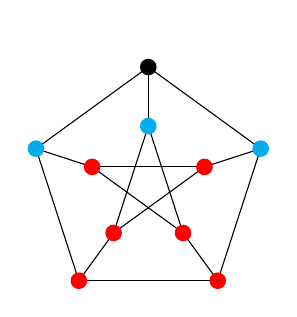
\begin{tikzpicture}
  \coordinate (center) at (1,2);
  \def\radius{.75cm}
  \def\rad2{1.5cm}
  
  \coordinate (o0) at (0*360/5+90:\radius);
  \coordinate (o1) at (1*360/5+90:\radius);
  \coordinate (o2) at (2*360/5+90:\radius);
  \coordinate (o3) at (3*360/5+90:\radius);
  \coordinate (o4) at (4*360/5+90:\radius);

  \coordinate (i0) at (0*360/5+90:\rad2);
  \coordinate (i1) at (1*360/5+90:\rad2);
  \coordinate (i2) at (2*360/5+90:\rad2);
  \coordinate (i3) at (3*360/5+90:\rad2);
  \coordinate (i4) at (4*360/5+90:\rad2);
  
  \draw (i0) -- (i1);
  \draw (i1) -- (i2);
  \draw (i2) -- (i3);
  \draw (i3) -- (i4);
  \draw (i4) -- (i0);
  
  \draw (o0) -- (o2);
  \draw (o0) -- (o3);
  \draw (o1) -- (o3);
  \draw (o1) -- (o4);
  \draw (o2) -- (o4);
   
  \draw (i0) -- (o0);
  \draw (i1) -- (o1);
  \draw (i2) -- (o2);
  \draw (i3) -- (o3);
  \draw (i4) -- (o4);
  
  \fill[cyan] (center) (o0) circle[radius=3pt];
  \fill[red] (center) (o1) circle[radius=3pt];
  \fill[red] (center) (o2) circle[radius=3pt];
  \fill[red] (center) (o3) circle[radius=3pt];
  \fill[red] (center) (o4) circle[radius=3pt];

  \fill[black] (center) (i0) circle[radius=3pt];
  \fill[cyan] (center) (i1) circle[radius=3pt];
  \fill[red] (center) (i2) circle[radius=3pt];
  \fill[red] (center) (i3) circle[radius=3pt];
  \fill[cyan] (center) (i4) circle[radius=3pt];
  
\end{tikzpicture}
\caption{Petersen graph $G$}
%\label{petersen}
\end{subfigure}
\begin{subfigure}{.5\textwidth}
\centering
\begin{tikzpicture}
  \coordinate (v1) at (0,-0.5);
  \coordinate (v2) at (1.5,-0.5);
  \coordinate (v3) at (3,-0.5);
  \coordinate (v3_eps) at (3.25,-0.5);
  \coordinate (loop_label) at (3.65,-0.2);

  \draw (v1) node[below] {$v_1$};
  \draw (v2) node[below] {$v_2$};
  \draw (v3) node[below] {$v_3$};
  
  \draw (v1) -- node[above]{1} (v2);
  \draw (v2) -- node[above]{2} (v3);
  
  \draw (loop_label) node {4};
  
  \draw[black] (v3_eps) circle[radius=6pt];
  
  
  \filldraw[white] (0,1.05) circle[radius=3pt];
  \filldraw[white] (0,-2.1) circle[radius=3pt];
  
  \filldraw[black] (v1) circle[radius=3pt];
  \filldraw[cyan] (v2) circle[radius=3pt];
  \filldraw[red] (v3) circle[radius=3pt];
   
  
%  \[red] (cyan) (o3) circle[radius=3pt];
%  \fill[red] (red) (o3) circle[radius=3pt];
\end{tikzpicture} 
\caption{Graph $G'$}
\label{petersen_a}
\end{subfigure}
\caption{The Petersen graph $G$ and a three vertex weighted graph which it covers.  In the covering map, vertices in $G$ are sent to the vertex with same color in $G'$.\label{petersen}}
\end{figure}

% NOTE(Josh): Can use this later
% \noindent \textbf{Example.}  Consider an even cycle $C_{2n}$, and let $P_{n+1}$
% be the path of length $n+1$.  Then $P_{n+1}$ is a projection of $C_{2n}$.  We
% construct the covering map $\pi$ as follows. 
% 
% 
% Let $d(x,y)$
% be the length of a shortest path from vertex $x$ to vertex $y$ in $C_{2n}$.  
% Denote the vertices of the path by $v_0, v_1, \cdots, v_{n}$, where $v_i$
% is adjacent to $v_{i+1}$.
% Now for any fixed vertex $x$ in $C_{2n}$, we can define the map 
% $\pi : V(C_{2n}) \to V(P_{n+1})$, where $\pi$ sends vertex $y$ to the 
% vertex $v_{d(y,x)}$.  This is a covering map with index $m=2$.  
  
%%%%%%%%%%%%%%%%%%%%%%%%%%%%%%%%%%%%%%%%%%%%%%%%%%%%%%%%%%%%%%%%%%%%%%%%%%
%% SECTION FOUR
%%%%%%%%%%%%%%%%%%%%%%%%%%%%%%%%%%%%%%%%%%%%%%%%%%%%%%%%%%%%%%%%%%%%%%%%%%

\section{Spectral Gap of Graphs in $\mathcal{F}_n$}

\subsection{A Projection of Graphs in $\mathcal{F}_n$}

We begin by constructing a weighted graph $G_n$ on three vertices, which is
a projection of every graph in $\mathcal{F}_n$.  Then we compute the 
eigenvalues of $G_n$, and by Corollary~\ref{cor:cov-cor}, these will be 
eigenvalues of every graph in $\mathcal{F}_n$.  
Let $F$ be a graph in $\mathcal{F}_n$, and 
let $G_n$ be the weighted graph with vertices $\{v_1, v_2, v_3\}$,
with edge weights $w(v_1,v_1) = n-2$, $w(v_1,v_2) = 1$, $w(v_2, v_3) = n-2$,
$w(v_3,v_3) = (n-2)^2$, and all other edge weights zero.
To construct the covering map $\pi : V(F) \to V(G_n)$, we just need to 
specify the sets $U_1 = \pi^{-1}(v_1), U_2 = \pi^{-1}(v_2), U_3 = \pi^{-1}(v_3)$: 
\begin{eqnarray*}
 U_1 = \pi^{-1}(v_1) & = & \{\tau \in S_n : \tau_n = n \} \\
 U_2 = \pi^{-1}(v_2) & = & \{\tau \in S_n : \tau_1 = n \} \\
 U_3 = \pi^{-1}(v_3) & = & \{\tau \in S_n : \tau_1 \neq n, \tau_n \neq n \}  
\end{eqnarray*}


\noindent In order to verify that this is a covering, we need to check the two properties:
\begin{itemize}
\item[(1)]  We need to show that any two vertices in the same preimage set $U_i$ have
  the same number of neighbors in each preimage set $U_j$.  For example, take
  $\tau \in U_3$, so $\tau_k = n$ for some $1 < k < n$.  By definition of
  $\mathcal{F}_n$, if $\sigma$ is adjacent to $\tau$ then either
  $\sigma_n = \tau_n$ or $\sigma_n = \tau_1$.  In particular,
  $\sigma_n \neq n$, so $\tau$ is not adjacent to any vertex in $U_1$.
  There is exactly one neighbor of $\tau$ with $\sigma_1 = n$, and
  so $\tau$ is adjacent to exactly one vertex in $U_1$.  The remaining
  $n-2$ neighbors of $\tau$ are in $U_3$.  As required, the number of neighbors in each
  preimage set did not depend on the choice of $\tau \in U_3$.
  The cases that $\tau \in U_1$ and $\tau \in U_2$ are similar.
 
 \item[(2)]  We need to verify equation~\ref{covering_sum_condition} for each
   pair chosen from the preimage sets $U_1, U_2, U_3$.  
 For this covering, we have $m=(n-1)!$. 
 Firstly, $U_1$ and $U_1$:
  \[ \sum_{\substack{x \in U_1 \\ y \in U_1}} w(x,y) = \sum_{x \in U_1} (n-2)\]
 since each element of $U_1$ is adjacent to exactly $n-2$ elements in $U_1$.
 So 
  \[ \sum_{\substack{x \in U_1 \\ y \in U_1}} w(x,y) = |U_1| (n-2) = (n-1)! w(v_1,v_1)\]
 as required.  The pairs $U_1$, $U_2$ and $U_2$, $U_3$ are similarly verified.
 
% Next, $U_1$ and $U_2$:
 %  \[ \sum_{\substack{x \in U_1 \\ y \in U_2}} w(x,y) = \sum_{x \in U_1} 1 = (n-1)! w(v_1, v_2) .\]
 For the pair $U_1$ and $U_3$, since there are no edges between these sets
and since $w(v_1,v_3) = 0$, we are done.  Similarly for the pair $U_2$ and $U_2$.
 %For $U_2$ and $U_3$ we have 
 %\[\sum_{\substack{x \in U_2 \\ y \in U_3}} w(x,y) = \sum_{x \in U_1} (n-2) = (n-1)! w(v_2, v_3) . \]
 And finally, the pair $U_3, U_3$:
  \[\sum_{\substack{x \in U_3 \\ y \in U_3}} w(x,y) = \sum_{x \in U_3} (n-2) = |U_3|(n-2)\]
 Now  $|U_3| = n! - |U_1| - |U_2| = (n-2) (n-1)!$, so we get
  \[\sum_{\substack{x \in U_3 \\ y \in U_3}} w(x,y)  = (n-1)! w(v_3,v_3)\]
 as required.  
 
\end{itemize}
Now that we have a covering, we evaluate the eigenvalues of the projection $G_n$.

\begin{lemma}
\label{g_eigen}
The eigenvalues of the normalized Laplacian  of $G_n$ are \\$0, \frac 1{n-1}, \frac n {n-1}$.  
\end{lemma}
\begin{proof}
% The adjacency matrix of $G_n$ is 
% \[ \left[ \begin{array}{ccc}  n-2 & 1 & 0\\
%                              1 & 0 & n-2 \\
%                             0 & n-2 &  (n-2)^2
%                              \end{array} \right] \]
The normalized Laplacian of $G_n$ is
                              \[ \left[ \begin{array}{ccc}  \frac 1 {n-1} &- \frac 1 {n-1} & 0\\
                             - \frac 1 {n-1} &1 &- \frac{\sqrt{n-2}}{n-1} \\
                             0 &  -\frac{\sqrt{n-2}}{n-1} &  \frac 1 {n-1}
                              \end{array} \right] \]
 The result follows from a simple computation.
\end{proof}

\begin{corollary}\label{cor:adj_spec}
For any $G \in \mathcal{F}_n$, the adjacency matrix $A_{G}$ has eigenvalues $n-1$, $n-2$ and $-1$.
For $1 \leq i \leq n$ define
\begin{eqnarray*}
 X(i) & = & \{\tau \in S_n : \tau_n = i \} \\
 Y(i) & = & \{\tau \in S_n : \tau_1 = i \} \\
 Z(i) & = & \{\tau \in S_n : \tau_1 \neq i, \tau_n \neq i \}  
\end{eqnarray*}
Then any eigenfunction corresponding to any other eigenvalue than those listed above must sum to zero on
each of $X(i)$, $Y(i)$ and $Z(i)$, for any $i \in \{1,2,\cdots,n\}$.
\end{corollary}
\begin{proof}
  When defining the covering mapping $\pi$ to $G_n$, for
  a permutation $\tau$ the vertex it was mapped to was
  determined by the position of $n$ in $\tau$. 
  Observe that we can replace $n$ with any index $i$, $1 \leq i \leq n$, and
  we still have a covering, in this case with preimage sets $X(i)$, $Y(i)$, $Z(i)$.


  Now take an eigenfunction of $G$ which corresponds to an eigenfunction other than
  $n-1$, $n-2$, or $-1$.  $G$ is regular, so this eigenfunction is also an
  eigenfunction of the normalized Laplacian of $G$, corresponding to an eigenvalue
  other than $0$, $1/(n-1)$ or $n/(n-1)$.  It follows from Corollary~\ref{cor:cov-cor}
  and the previous lemma that the eigenfunction must sum to zero over the preimage
  sets of the covering, which are $X(i)$, $Y(i)$ and $Z(i)$.    
\end{proof}

%%%%%%%%%%%%%%%%%%%%%%%%%%%%%%%%%%%%%%%%%%%%%%%%%%%%%%%%%%%%%%%%%%%%%%%%%%
%% SECTION FIVE
%%%%%%%%%%%%%%%%%%%%%%%%%%%%%%%%%%%%%%%%%%%%%%%%%%%%%%%%%%%%%%%%%%%%%%%%%%


\subsection{The Spectral Gap is $1$}

Recall that $\mathcal{F}_n$ is the family of graphs whose vertex set is $S_n$ and
where for each vertex $\tau$,
\[ \tau = (\tau_1, \tau_2, \cdots, \tau_n), \]
and each $2 \leq i \leq n$, $\tau$ is adjacent to exactly one vertex of the form 
\[ (\tau_i, \alpha_2, \alpha_3, \cdots, \alpha_{i-1}, \tau_1, \tau_{i+1}, \cdots, \tau_n). \]
Each graph in $\mathcal{F}_n$ is an $(n-1)$-regular graph.  The prefix reversal graph $\mathcal{P}_n$
is in $\mathcal{F}_n$, as well as the right-Cayley graph generated by the transpositions $(1\ k)$,
where $2 \leq k \leq n$.


In order to compute the spectral gap of graphs in $\mathcal{F}_n$, we proceed
by induction, so first we compute the spectrum of graphs in $\mathcal{F}_3$ to 
establish our base case.  

\begin{lemma}\label{base_case}
  $\mathcal{F}_3 = \{ C_6 \}$.  In particular, the adjacency spectral gap of every graph in
  $\mathcal{F}_3$ is one.
\end{lemma}
\begin{proof}
  Let $G \in \mathcal{F}_3$.  Then $G$ is a $2$-regular graph on $3! = 6$ vertices.
  From the definition of $\mathcal{F}_3$, it is easy to verify that $G$ is connected,
  and so $G = C_6$.  The first two adjacency eigenvalues of $C_6$ are $2$ and $1$.
\end{proof}

%\begin{theorem}
%  For $n \geq 3$, and any $G \in \mathbb{P}_n$, the spectral gap of $\mathcal{L}_{G}$ is $1/(n-1)$, and the spectral
%  gap of $A_{G}$ is $1$.

We can now prove the  theorem on the spectral gap of ${\mathcal F}_n$, as stated in the Section~1.

%\end{theorem}
\begin{proof}[Proof of Theorem~\ref{thm:main}]
  We proceed by induction,
  so assume that the adjacency spectral gap of any graph in $\mathcal{F}_{n-1}$ is $1$.  
  The base case is established by Lemma~\ref{base_case}.  By $(n-2)$-regularity of graphs
  in $\mathcal{F}_{n-1}$, it follows from the inductive assumption that the second largest
  eigenvalue of any graph in $\mathcal{F}_{n-1}$ is $n-3$.


  Let $G$ be a graph in $\mathcal{F}_{n}$.
  Pick any eigenvector $f$ coming from an eigenvalue $\mu$ that is not
  $n-1$, $n-2$ or $-1$.  Our goal is to show that $\mu < n-2$.
  Recall that $X(i)$ consists of the permutations whose 
  last entry is $i$, $Y(i)$ consists of the permutations whose first entry is
  $i$ and $Z(i)$ consists of all other permutations.  For any $i$, from 
  Corollary~\ref{cor:adj_spec}
  we get a projection of $G$ with preimage sets 
  $X(i), Y(i), Z(i)$.
  The set $X(i)$ induces a graph in $\mathcal{F}_{n-1}$, and the set $Y(i)$
  induces an independent set (since every two adjacent permutations have
  different first entries).
  Furthermore the edges between $X(i)$ and 
  $Y(i)$ form a matching.  Our proof strategy is the following:  we will
  get an expression for $\mu$ involving the values of $f$ on the 
  set $X(i)$ and the set $Y(i)$.  We can control the contribution from 
  $X(i)$ using the inductive assumption, and then we show that we can
  choose $i$ so that the contribution from $Y(i)$ is small enough
  to yield the stated result.
  
  
  \vspace*{1mm}
  \noindent \textbf{Claim:} We can fix an $i$ such that 
   \begin{equation}\label{eqn:gap_max}
     \sum_{x \in X(i)} f(x)^2 \geq \sum_{y \in Y(i)} f(y)^2
   \end{equation}
   and 
   \[ \sum_{x \in X(i)} f(x)^2 > 0. \]
   \textbf{Proof of claim:} Notice that the sets $X(1), X(2), \cdots, X(n)$
  partition the vertex set of $G$ (ie.  partitioning the permutations
  based on the last entry).  Similarly, the sets 
  $Y(1), Y(2), \cdots, Y(n)$ partition the vertex set of $G$.
  Hence
   \[ \sum_{j=1}^n \sum_{x \in X(j)} f(x)^2 = \sum_{j=1}^n \sum_{y \in Y(j)} f(y)^2 >0 . \]
  In particular, there exists an index $i$ such that 
   \begin{equation*}
     \sum_{x \in X(i)} f(x)^2 \geq \sum_{y \in Y(i)} f(y)^2.
   \end{equation*}
Let $I$  denote the set of indices $i$ satisfying the above inequality. Then there exists some $i$ in $I$ satisfying
   \begin{equation*}
     \sum_{x \in X(i)} f(x)^2 > 0
   \end{equation*}
  since $f \not = 0$. This proves the claim.
  
  
  
  Consider an arbitrary vertex $x \in X(i)$.  Then by
  definition of $X(i)$, $x$
  is a permutation with $x(n) = i$.
  $x$ has $n-1$ neighbors in $G$, $n-2$ of these neighbors
  are in $X(i)$ and one of its neighbors is in $Y(i)$.
  Let $c_x$ be the unique neighbor of $x$ in $Y(i)$.
  As noted above, the induced subgraph on $X(i)$ is in $\mathcal{F}_{n-1}$.
  By the eigenvalue-eigenvector equation, we have
   \[ \mu f(x) = f(c_x) + \sum_{y \in N(x) \cap X(i)} f(y) .\]
  Multiplying both sides by $f(x)$, and summing over $x \in X(i)$
  yields
   \[ \mu \sum_{x \in X(i)} f(x)^2 = \sum_{x \in X(i)} f(x) f(c_x) + \sum_{x \in X(i)} \sum_{y \in N(x) \cap X(i)} f(x) f(y) .\]
  Dividing across by the sum on the left-hand side (which is non-zero 
  by our claim above) gives
   \begin{equation}\label{eqn:gap_to_bound}
     \mu = \frac{\sum_{x \in X(i)} f(x) f(c_x)}{\sum_{x \in X(i)} f(x)^2} + \frac{\sum_{x \in X(i)} \sum_{y \in N(x) \cap X(i)} f(x) f(y)}{\sum_{x \in X(i)} f(x)^2} .
    \end{equation}
  We will now find upper bounds for each of the two terms on
  the right-hand side.
  
  Let ${G'}$ be the induced subgraph on $X(i)$, which is a graph in $\mathcal{F}_{n-1}$, and let
  $g = f|_{X(i)}$.
  Since $\sum_{x \in X(i)} f(x)=0$, we have that $g \perp \textbf{1}$, where $\textbf{1}$ is the constant vector with entries $1$,
  which is the eigenvector associated with $\mu_1$.
  Now we can bound the second term in equation~\ref{eqn:gap_to_bound} by $n-3$:
     \begin{eqnarray*}
     \displaystyle \frac{\displaystyle\sum_{x \in X(i)} \displaystyle\sum_{y \in N(x) \cap X(i)} f(x) f(y)}{\displaystyle\sum_{x \in X(i)} f(x)^2} & = & \frac{g^T A_{G'} g}{ g^T g} \\
     &\leq& \text{max}_{h \perp \textbf{1}} \frac{h^T A_{G'} h}{h^T h} \\
     &=& \mu_2(G') \\
     &=& n-3.
   \end{eqnarray*}
 
 



   The edges between $X(i)$ and $Y(i)$ are a matching.
  So as $x$ ranges over the vertices of $X(i)$, $c_x$ ranges over
  the vertices of $Y(i)$.  By Cauchy--Schwarz,
   \begin{eqnarray*} 
   \sum_{x \in X(i)}f(x) f(c_x) & \leq & \sqrt{\sum_{x \in X(i)}f(x)^2 \sum_{x \in X(i)}f(c_x)^2 } \\
   & = & \sqrt{\sum_{x \in X(i)}f(x)^2 \sum_{y \in Y(i)}f(y)^2 } 
   \end{eqnarray*}
  So
   \[ \frac{\displaystyle \sum_{x \in X(i)} f(x) f(c_x)}{\displaystyle \sum_{x \in X(i)} f(x)^2} \leq \sqrt{\frac{\displaystyle \sum_{y \in Y(i)}f(y)^2}{\displaystyle {\sum_{x \in X(i)}f(x)^2}}} \leq 1 \]
  where the last inequality follows from equation~\ref{eqn:gap_max}.
   
  Applying these two bounds in equation~\ref{eqn:gap_to_bound} gives
  \[ \mu \leq n-3 + 1 = n-2 . \]
  This shows that there is no eigenvalue of $G$ strictly between $n-2$ and $n-1$, so
  we conclude that  $\mu_2(G) = n-2$.
\end{proof}


As a brief application of Theorem~\ref{thm:main}, we can establish bounds on the edge
expansion of every graph in $G \in \mathcal{F}_n$.  Recall that the edge
expansion of a $d$-regular graph $G$, $h_G$, is defined as
\[ h_G = \min_{S \subset V(G)} \frac{|E(S,\bar{S})|}{\min(|S|,|\bar{S}|) \cdot d} .\]
If $S$ is the set of permutations whose last entry is $n$, then
$|S| = |E(S,\bar{S})| = (n-1)!$, which gives the upper bound
$h_G \leq 1/(n-1)$.  To obtain a lower bound, we can use an inequality
from \cite{Chung1997},
$h_G \geq \lambda_1 / 2$.   Combining these two inequalities gives the bounds
 \[ \frac{1}{2(n-1)} \leq h_G \leq \frac{1}{n-1} .\] 


%%%%%%%%%%%%%%%%%%%%%%%%%%%%%%%%%%%%%%%%%%%%%%%%%%%%%%%%%%%%%%%%%%%%%%%%%%
%% SECTION SIX
%%%%%%%%%%%%%%%%%%%%%%%%%%%%%%%%%%%%%%%%%%%%%%%%%%%%%%%%%%%%%%%%%%%%%%%%%%

\section{The Reversal Graph}\label{s6}

\subsection{A Graph Projection of the Reversal Graph}

The graph $R_n$ is a Cayley graph of $S_n$ that does not
belong to the family $\mathcal{F}_n$ but is closely related.  For any 
$1 \leq i<j \leq n$, let $r_{i,j}$ denote the bijection on $S_n$
defined by
 \[ r_{i,j}(\tau) =  (\tau_1, \tau_2, \cdots, \tau_{i-1}, \tau_{j}, \tau_{j-1}, \cdots \tau_{i+1}, \tau_i, \tau_{j+1}, \cdots , \tau_{n})\] 
That is, it reverses the subsequence from indices $i$ to $j$, inclusive.
Then two permutations $\sigma$ 
and $\tau$ are adjacent in $R_n$ iff $\tau = r_{i,j}(\sigma)$ for some $i< j$.  We will first  show that $R_n$ has many integer eigenvalues.  We remark that the spectrum of $R_n$ is not generally
integer-valued, despite the presence of many integer eigenvalues.  A plot of
the $7!$ eigenvalues of $R_7$ is given in Figure~\ref{fig-spec7}.  We will first prove the following useful fact.


\begin{figure}[h]
\begin{center}
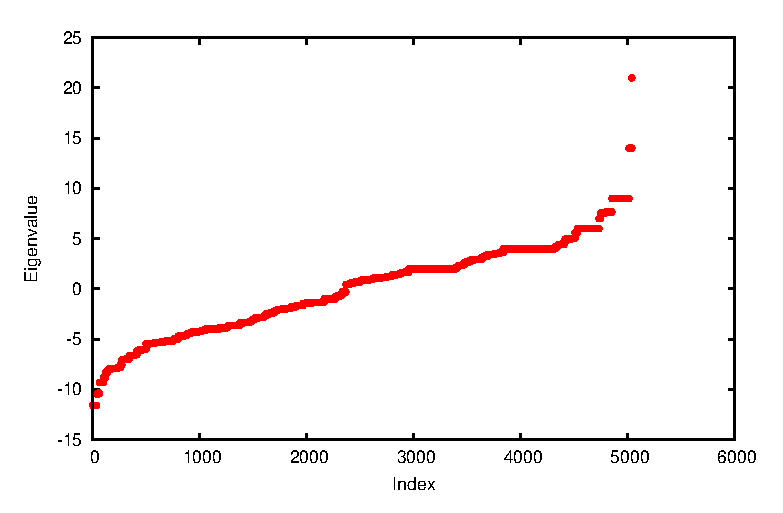
\includegraphics[scale=.85]{figures/all_spec7.eps} 
\end{center}
\caption{The adjacency eigenvalues of the reversal graph, $R_7$, plotted in increasing order.
  \label{fig-spec7}}
\end{figure}


\begin{lemma}\label{lem:rev_eig}
Let $X$ be the symmetric $n \times n$ matrix with entries
 \[ X_{i,j} = \text{min} \left\{ i,j,n+1-i,n+1-j \right\} \]
For a given real number $x$, let $D$ be the unique diagonal matrix such 
that every row of $D+X$ sums to $x$.  Then the eigenvalues of $D+X$ are
\[ \mu_k =  x - \left\lfloor \frac{k}{2} \right\rfloor n + 2 \binom{\left \lfloor \frac{k}{2} \right \rfloor}{2}, 1 \leq k \leq n . \]
In particular, $\mu_1 = x$, $\mu_2 = x-n$.
%   \[x, x-n, x - n - (n-2),  \cdots, x - n - (n-2) - \cdots - \left(n - 2 \left\lfloor \frac{n}{2} \right\rfloor\right)\]
\end{lemma}


\noindent \textbf{Example: } For $n=5$ and $x=12$ we get
\[ D+X = \begin{pmatrix}
 7 & 0 & 0 & 0 & 0 \\
 0 & 4 & 0 & 0 & 0 \\
 0 & 0 & 3 & 0 & 0 \\
 0 & 0 & 0 & 4 & 0 \\
 0 & 0 & 0 & 0 & 7 
\end{pmatrix}
+ \begin{pmatrix}
 1 & 1 & 1 & 1 & 1 \\
 1 & 2 & 2 & 2 & 1 \\
 1 & 2 & 3 & 2 & 1 \\
 1 & 2 & 2 & 2 & 1 \\
 1 & 1 & 1 & 1 & 1 
\end{pmatrix} \]
which has eigenvalues $12, 7, 7, 4, 4$.


\begin{proof}
 We proceed by induction.  For the case $n=1$, the result is immediate.  
 When $n=2$, we have
  \[ D+X = \begin{pmatrix}
 x-1 & 1 \\
 1 & x-1
\end{pmatrix} \]
which has eigenvalues $x$ and $x-2$, as required.

Now fix $n$ and assume the result holds for all smaller dimensions. 
Since $D+X$ is a symmetric matrix with constant row sums, the leading 
eigenvector of $D+X$ is
the all-ones vector $\textbf{1}$, with corresponding eigenvalue 
$x$.  All other eigenvectors are orthogonal to $\textbf{1}$.
It follows that if $Y = D+X - \textbf{1}\textbf{1}^T$,
then $D+X$ and $Y$ have the same eigenvectors.   Moreover, 
the spectrum of $Y$, counting multiplicity, is exactly the
spectrum of $D+X$ with $x$ replaced by $x-n$.


The only non-zero entry in the top row of $Y$ is the top-left entry, which
is $x-n$.  The only non-zero entry in the bottom row of $Y$ is the bottom-right entry which is also $x-n$.
Denote the characteristic polynomial of a matrix $A$ by $p_A(\mu)$.  Expanding the determinant of $Y - \mu I$
along the top row and then along the bottom row, we obtain that 
 \[ p_Y(\mu) = (\mu - x + n)^2 p_{Y'}(\mu) \]
where $Y'$ is the $(n-2) \times (n-2)$ principal submatrix of $Y$, obtained
by deleting the first and last rows and columns.  In particular, the spectrum
of $Y$ consists of $x-n$ with multiplicity two, and the spectrum of $Y'$.
Hence, from the relationship between the spectrum of $D+X$ and the spectrum of
$Y$ discussed above, we  have that the eigenvalues of $D+X$ are exactly
the eigenvalues of $Y'$, together with $x$ and $x-n$.


Observe that $Y'$ satisfies the conditions of the theorem, with row sum equal 
to $x-n$.  By induction, we have that the eigenvalues of $Y'$ are (for $1 \leq k \leq n-2$):
\begin{eqnarray*}
  \mu_k(Y') & = & (x-n) - \left\lfloor \frac{k}{2} \right\rfloor (n-2) + 2 \binom{\left\lfloor \frac{k}{2} \right\rfloor}{2} \\
  & = & x - \left\lfloor \frac{k+2}{2} \right\rfloor n + 2 \binom{\left\lfloor \frac{k+2}{2} \right\rfloor}{2} .
\end{eqnarray*}
Combining these $n-2$ eigenvalues with $x$ and $x-n$ yields exactly the claimed spectrum for $D+X$.
\end{proof}

\begin{lemma}\label{lem:rev_eig2}
  The spectrum of the adjacency matrix of the reversal graph, $A_{R_n}$, 
  contains the eigenvalues
\[ \mu_k =  \binom{n}{2} - \left\lfloor \frac{k}{2} \right\rfloor n + 2 \binom{\left \lfloor \frac{k}{2} \right \rfloor}{2}, 1 \leq k \leq n . \]
%   \[\binom{n}{2}, \binom{n}{2}-n, \binom{n}{2} - n - (n-2),  \cdots, \binom{n}{2} - n - (n-2) - \cdots - \left(n - 2 \left\lfloor \frac{n}{2} \right\rfloor\right)\]
  In particular, $\binom{n}{2}$ and $\binom{n}{2} - n$ are eigenvalues, and so the spectral gap is at most $n$. 
\end{lemma}  

\begin{proof}
  We begin by constructing a projection of the graph $R_n$.
  Let $G$ be the graph with vertices $v_1$, $v_2$, $\cdots$,
  $v_n$ corresponding to the adjacency matrix $A_G = D+X$,
  where vertex $v_i$ corresponds to row and column $i$, and
  $D+X$ is as in the previous lemma, with row sum $\binom{n}{2}$.
  Let $U(i)$ be the set of all permutations $\tau$ such that $\tau_i = n$.
  The sets $U(i)$, for $1\leq i \leq n$, partition $V(R_n)$, so we
  can define a map $\pi : V(R_n) \to V(G)$ by
  setting $\pi(x) = v_i$ whenever $x \in U(i)$.  It suffices to show
  that this is a covering map, then the result will follow
  from the previous lemma.


  To show that $\pi$ satisfies the first property of a graph cover,
  we need that for all indices $i,j$, any two vertices in $U(i)$
  have the same number of neighbors in $U(j)$.  This follows from the
  fact that there are a fixed number of reversals that map
  entry $i$ to entry $j$.

%  Firstly,
%  assume that $i < j$.  Then the reversals that map
%  a vertex in $U(i)$ to $U(j)$ are exactly
%  $r_{i,j}, r_{i-1,j+1}, r_{i-2,j+2}, \cdots$.  It follows that
%  any vertex in $U(i)$ is adjacent to exactly
%  $\text{min}\left\{i,j,n+1-i,n+1-j\right\}$ vertices in $U(j)$.
%  Similarly if $j < i$.
%  Secondly, assume $i = j$.  For any vertex in $U(i)$,
%  there are several types of reversals that map it back into $U(i)$:
%  the reversals $r_{j,k}$ where $j < k < i$; the reversals 
%  $r_{j,k}$ where  $i < j < k$; and finally the reversals of the form
%  $r_{i-k,i+k}$.  In every case, all vertices in $U(i)$ have
%  the same number of neighbors in $U(j)$.


  For the second property, take two preimage sets $U(i)$, $U(j)$,
  and $\tau_0$ some permutation in $U(j)$.  It is easily checked
  that by construction of the weighted graph $G$, we have
  \[ w(v_i, v_j) = \left| N(\tau_0) \cap U(i) \right| .\]
  Then
  \begin{eqnarray*}
    \displaystyle \sum_{\sigma \in U(i)} \sum_{\tau \in U(j)} w(\sigma,\tau) & = & \sum_{\sigma \in U(i)} |U(j)| w(\sigma,\tau_0) \\
    & = & (n-1)! \left| N(\tau_0) \cap U(i) \right|  \\
    & = & (n-1)! w(v_i, v_j)
  \end{eqnarray*}
  where the first equality follows from property (i).
  Hence $\pi$ is a covering with $m = (n-1)!$.

  %CURP
  
%  Consider a vertex $\tau$ in 
%$U(i)$, and any index $j > i$.  The reversals that map $\tau$ into 
%$U(j)$ are exactly $r_{i,j}, r_{i-1,j+1}, r_{i-2,j+2}, \cdots$.   It
%follows that the  number of vertices in $U(j)$ that are adjacent 
%to $\tau$ is $\text{min}\left\{i,j,n+1-i,n+1-j\right\}$.  This is independent
%of the vertex $\tau$ chosen.  Similarly, we get the same total
%when $j < i$.  In particular any two vertices in $U(i)$
%have the same number of neighbors in $U(j)$, for any $j \neq i$.  
%
%There are several types of reversals that map $\tau$ back into $U(i)$.  They
%are: the reversals $r_{j,k}$ where $j < k < i$, the reversals 
%$r_{j,k}$ where  $i < j < k$, and finally the reversals of the form
%$r_{i-k,i+k}$.  Again, the number of such reversals does not depend on the 
%vertex $\tau$ chosen, and so any two vertices in $U(i)$ have the same number
%of neighbors in $U(i)$.  
%
%
%It follows from the above two paragraphs that we can form a projection of 
%the graph $R_n$ on $n$ vertices, with preimage sets $U(i)$.  The 
%adjacency matrix of this projection can be written as $D+X$, where 
% \[ X(i,j) = \text{min}\left\{i,j,n+1-i,n+1-j\right\} \] 
%and $D$ is the unique diagonal such that $D+X$ has constant row sum equal
%to $\binom{n}{2}$.  By Corollary~\ref{cor:cov-cor}, the eigenvalues
%of $D+X$ are eigenvalues of $A_{R_n}$.  The result then follows from 
%Lemma~\ref{lem:rev_eig}.
\end{proof}

\subsection{The Spectral Gap of the Reversal Graph}

We are finally ready to prove the main theorem determining the spectral gap of $R_n$.

\noindent
{\it Proof of Theorem \ref{thm:rev_eig}:}
 The value of $\mu_1$ is $\binom n 2$ since $R_n$ is regular of degree $\binom n 2$.   
 From the previous lemma we have that 
  \[ \mu_2 \geq \binom{n}{2} - n\]
 so it suffices to prove that
  \[ \mu_2 \leq \binom{n}{2} - n .\]
 We follow a similar approach to the proof of 
 Theorem~\ref{thm:main}.  
 
 
 We proceed by induction.  For the base case, consider $n=2$.  Then $R_2$
 is $K_2$, with eigenvalues $1,-1$.  Now assume for any $m < n$, we have
 \[  \mu_2(A_{R_m}) = \binom{m}{2} - m . \]
 For any $1 \leq i \leq n$, we define the sets
  \[ U_i(j) = \left\{ \tau \in S_n : \tau_j = i \right\}. \]
 As in the proof of Lemma~\ref{lem:rev_eig2}, for any fixed $i$ the sets 
 $U_i(j)$, $1 \leq j \leq n$ are the preimages of a covering map of $R_n$,
 and the two largest eigenvalues of the projection are $\binom{n}{2}$ and
 $\binom{n}{2} - n$.  It follows from Corollary~\ref{cor:cov-cor}
 that if $A_{R_n}$ has an eigenvalue $\mu$ strictly between $\binom{n}{2}$
 and $\binom{n}{2} - n$ then the corresponding eigenvector must sum to zero
 on $U_i(j)$ for all $i,j$.  Let $\mu$ be such an eigenvalue, with 
 eigenvector $f$.
 
 
 Let $E_1 = \left\{ \left\{\sigma, \tau\right\} \in E(R_n) : \sigma_1 \neq \tau_1 \right\}$,
 that is, the set of edges arising from substring reversals that include 
 the first entry of the permutation.  Observe that the edge set $E_1$
 is exactly the set of edges of the prefix reversal graph $\mathcal{P}_n$.
 Let $R'$ be the graph obtained by removing all edges in $E_1$ from $R_n$.  Then
 $R'$ consists of $n$ connected components, $U_1(1), U_2(1), \cdots, U_n(1)$.
 Each of these connected components is isomorphic to $R_{n-1}$.  
 
 
We have, by the Rayleigh quotient
  \begin{eqnarray*}
   \mu & = &  \frac{2\sum_{\{x,y\} \in E(R_n)} f(x) f(y)}{\sum_{x \in R_n} f(x)^2}\\
   & = & \frac{2\sum_{\{x,y\} \in E_1} f(x) f(y)}{\sum_{x \in R_n} f(x)^2} + \frac{2\sum_{\{x,y\} \not \in E_1} f(x)f(y)}{\sum_{x \in R_n} f(x)^2}\\
   & \leq & \mu_2(A_{\mathcal{P}_n}) + \frac{2\sum_{\{x,y\} \not \in E_1} f(x) f(y)}{\sum_{x \in R_n} f(x)^2}
   \end{eqnarray*}
 where the last inequality follows since $f$ is orthogonal to the constant
 vector $\textbf{1}$.  Using Theorem~\ref{thm:main} we have 
 $\mu_2(A_{\mathcal{P}_n}) = n-2$.
 
 
 To bound the second term, we will partition the edges not in $E_1$ in the following way
  \[ \left\{ \left\{ x,y \right\} \not \in E_1 \right\} = E(U_1(1)) \cup E(U_2(1)) \cup \cdots \cup E(U_n(1)) . \]
 Hence, we have 
  \begin{eqnarray*}
   \frac{2\sum_{\{x,y\} \not \in E_1} f(x) f(y)}{\sum_{x \in R_n} f(x)^2} & = & 
   \frac{\sum_{i=1}^n 2\sum_{\{x,y\} \in E(U_i(1))} f(x) f(y)}{\sum_{i=1}^n \sum_{x \in U_i(1)} f(x)^2} \\
   & \leq & \text{max}_{1 \leq i \leq n}  \frac{2\sum_{\{x,y\} \in E(U_i(1))} f(x) f(y)}{\sum_{x \in U_i(1)} f(x)^2} \\
   & \leq & \mu_2(A_{R_{n-1}}) 
  \end{eqnarray*}
 where we are using the fact that $v$ sums to zero over each set $U_i(1)$.
 Combining the two inequalities above, we get 
  \begin{eqnarray*}
  \mu & \leq & \mu_2(A_{\mathcal{P}_n}) + \mu_2(A_{R_{n-1}}) \\
  & = & (n-2) + \binom{n-1}{2} - (n-1) \\
  & = & \binom{n}{2} - n
  \end{eqnarray*}
  Thus we conclude that $\mu_2(A_{R_n}) = \binom n 2 -n$ and this completes the proof of Theorem \ref{thm:rev_eig}.
\qed



%%%%%%%%%%%%%%%%%%%%%%%%%%%%%%%%%%%%%%%%%%%%%%%%%%%%%%%%%%%%%%%%%%%%%%%%%%
%% SECTION SEVEN
%%%%%%%%%%%%%%%%%%%%%%%%%%%%%%%%%%%%%%%%%%%%%%%%%%%%%%%%%%%%%%%%%%%%%%%%%%

\section{Future Work}
Consider the stochastic process of pancake flipping:  Start with a stack of $n$ pancakes (or $n$ cards). At each
step, with probability $1/n$,  choose $i$ where $i=1, \ldots, n$ and  do a pancake flipping of the first $i$ pancakes. 

The above process is equivalent to taking a random walk on 
$\mathcal{P}_n + I$, where $\mathcal{P}_n$ is the pancake graph. The transition probability 
matrix is then $P=(A(\mathcal{P}_n)+I)/n$.

Since the first nontrivial eigenvalue of the normalized Laplacian of $\mathcal{P}_n$ is $1/(n-1)$. Consequently,
the first nontrivial eigenvalue of
the normalized Laplacian of $\mathcal{P}_n + I$ is $1/n$ and all eigenvalues of the normalized Laplacian
of $\mathcal{P}_n + I$ are at most $2-1/n$. It is known that the rate of convergence for random walk is the inverse of  $\lambda^{-1}$ where $\lambda= \min \{\lambda_1, 2-\lambda_{n-1}\}$ where $0=\lambda_0,
\lambda_1, \ldots, \lambda_{n-1}$ are the nontrivial eigenvalues of the normalized Laplacian of $\mathcal{P}_n + I$. However, in order to get tight bounds for the convergence of the random walk to the stationary distribution under the  total variational distance, more work is needed. For a vertex-transitive graph, a general upper bound after $t$ steps of random walk on 
$\mathcal{P}_n + I$ can be derived by using the Plancherel formula (see \cite{Chung1997}):
\begin{align*}
\Delta_{TV}(t) &\leq \frac 1 2 \Big( \sum_{i \not = 0} (1-\lambda_i)^{2t}\Big)^{1/2}.
\end{align*}
Using the result that $|1-\lambda_i| \leq 1-1/n$ for $i \not = 0$, we have
\begin{align*}
\Delta_{TV}(t) &< \frac 1 2 \Big(1-\frac 1 n\Big)^t n!\\
&\leq e^{-t/n+n \log n}.
\end{align*}
Hence, the random walk converges to the uniform distribution with $\Delta_{TV}(t) \leq e^{-c}$ after at most $t=n^2 \log n + c n$ steps.
If we know more about the distribution of eigenvalues $\lambda_i$, this upper bound should be improved.
It seems reasonable to conjecture that $O(n \log n)$ steps suffice.


Similarly, we can consider the random substring reversal process, where in each
step, with probability $\binom{n+1}{2}^{-1}$ we choose a substring (allowing substrings of length $1$) and reverse it.
This is equivalent to taking a random walk on $R_n+ nI$. 
In this case, we have $\lambda_1 = n/ \binom {n+1} 2= 2 (n+1)^{-1}$ and $\lambda_{n-1} \leq 2  - 2 (n+1)^{-1}$.   As in the case of 
pancake flipping, knowing the spectral gap allows us to obtain a bound on
the rate of convergence, but to obtain sharp bounds it would be desirable to
know more about the distribution of all eigenvalues.

We have mainly focused on substring reversal and pancake flipping on permutations. There are many
interesting variations of these problems. In particular, for applications such as genome
rearrangement, the objects of interest are signed permutations.  In this case the operation of
substring reversal is taking the reverse of the substring and changing the signs of every element in
the substring.  The corresponding problem for pancake flipping is the {\it burnt} pancake problem
where the sign is used to distinguish the two sides of each pancake.  The burnt pancake graph
$\bar{\mathcal P}_n$ has $2^n n!$ vertices and degree $n$.  A natural question is to determine
the spectral gap of the adjacency matrix.  In fact, $\mathcal{P}_n + I$ is a projection of
$\bar{\mathcal{P}}_n$, which implies that the adjacency spectral gap of $\bar{\mathcal{P}}_n$ is
at least one.  A natural guess is that the spectral gap of the adjacency matrix of
$\bar{\mathcal P}_n$ is exactly $1$. However, this
turns out to be not true. For $\bar{\mathcal P}_4$ the spectral gap is approximately $0.71343$,
and for $\bar{\mathcal P}_5$ the spectral gap is approximately $0.75758$.  



This chapter is based on the paper ``The Spectral Gap of Graphs Arising from Substring Reversals'',
submitted to \textit{Journal of Combinatorics}, written jointly with Fan Chung.  The dissertation
author was the primary investigator and author of the paper.
